% ============================================================
%  3. fejezet, KCMamba architektúra
% ============================================================
\chapter{A KCMamba architektúra}
\label{ch:architektura}

\section{Áttekintés}

A KCMamba (Kalman Core-Attention Mamba) egy hibrid neurális
architektúra, amely a Mamba SSM~\cite{gu2023mamba} rekurrens dinamikájába
egy differenciálható, tartalomfüggő Kalman-szűrő réteget integrál.
A modell nem rögzített $A$ felejtési faktorral dolgozik, hanem egy, a
bemenetből tanult $K$-gainből származtatott $A = 1-K$ együtthatót
használ az állapotfrissítésben. Ez lehetővé teszi, hogy az előzmény-
állapot és az aktuális megfigyelés közötti súlyozás a zajszintnek
megfelelően, adaptívan álljon be.

A modell két szintből épül fel: az alap feldolgozó egység a
\texttt{KCMambaBlock} (tartalom-függő Kalman-szűrés és állapotfrissítés),
fölötte a \texttt{KCMambaStack}: $N$ egymás utáni KC-blokk
cross-attention réteggel a végén.

\begin{figure}[H]
  \centering
  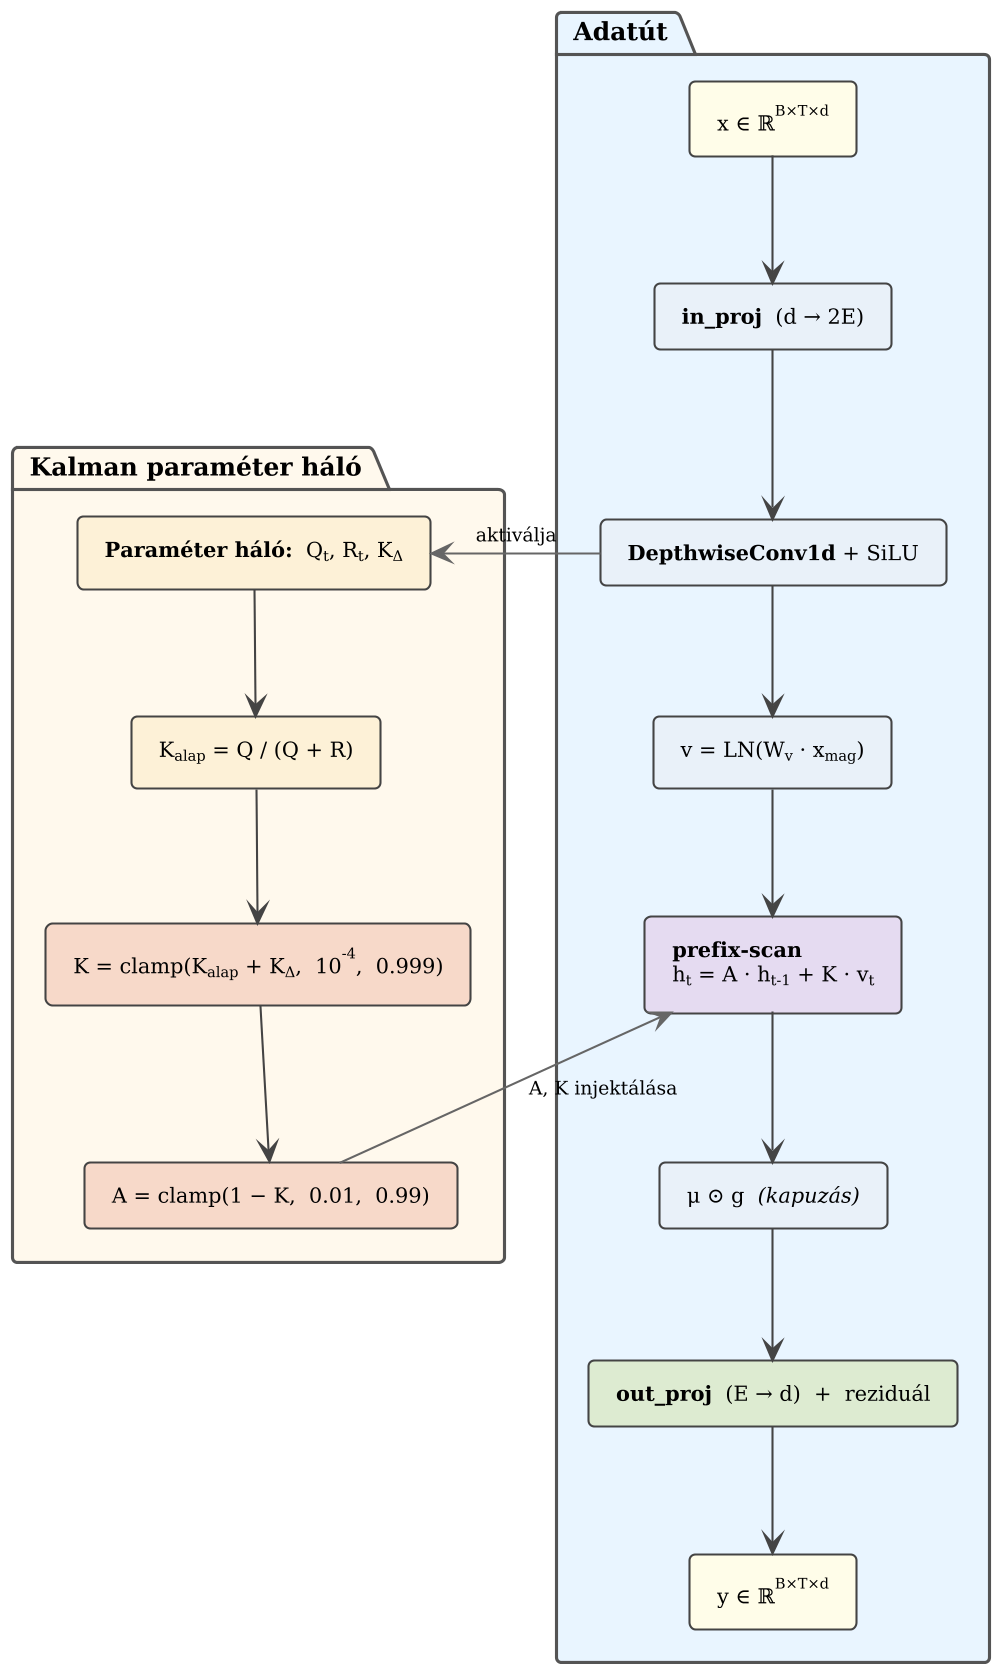
\includegraphics[width=\textwidth, height=0.85\textheight, keepaspectratio]{images/fig08_architecture_hu.png}
  \caption{A KCMamba blokk teljes adatfolyam-diagramja. A sárga blokkok
           ($Q_\text{net}$, $R_\text{net}$, $K_\text{net}$) tanítják a Kalman-statisztikákat,
           a lila blokkban történik a párhuzamos prefix-scan GPU-n $O(\log T)$
           szinkronizációval. A zöld blokkok a bemeneti és kimeneti projekciókat jelölik.}
  \label{fig:arch_overview}
\end{figure}

\section{KCMamba blokk}
\label{sec:kc_block}

Legyen a bemenő szekvencia $x \in \mathbb{R}^{B \times T \times d}$,
ahol $B$ a kötegméret, $T$ a szekvenciahossz, és $d$ a jellemzők száma.

\subsection{Bemeneti projekció és 1D-konvolúció}

A bemenetet két részre vetítjük egy lineáris réteggel,
majd SiLU aktivációs kapuzást alkalmazunk:
\begin{align}
    [x_\text{cw},\; x_\text{gate}] &= W_\text{in}\, x, \\
    \text{gate} &= \mathrm{SiLU}(x_\text{gate}),
\end{align}
ahol $W_\text{in} \in \mathbb{R}^{2d_\text{inner} \times d}$ a bemeneti projekciós
mátrix, $d_\text{inner}$ a belső csatornadimenzió, $x_\text{cw}$ a
Kalman-szűrési ághoz, $x_\text{gate}$ a kapuzáshoz továbbított csatorna,
és $\mathrm{SiLU}(z) = z \cdot \sigma(z)$ a Sigmoid Linear Unit aktiváció,
ahol $\sigma(z) = 1/(1+e^{-z})$ a logisztikus szigmoid.
A kétágú projekció két különböző szerepet tölt be.
Az $x_\text{cw}$ csatorna a Kalman-szűrési ág bemenete, míg az $x_\text{gate}$
csatorna a kimenet amplitúdójának független modulálásáért felel.
Ez a szétválasztás megakadályozza, hogy a kapuzási jel beavatkozzon a
Kalman-állapot dinamikájába.
A SiLU aktiváció ReLU-val szemben azért előnyös, mert sima és kis negatív
értékeket is megenged, ami a korai tanítás során javítja a gradiens-átmenetet.

A globális szekvenciális scan előtt az $x_\text{cw}$ csatornán egy depthwise
1D-konvolúció ($k=4$ kernel) biztosítja a lokális kontextus-integrációt:
\begin{equation}
    x_\text{core} = \mathrm{SiLU}\bigl(\mathrm{Conv1D}(x_\text{cw})\bigr).
\end{equation}
A konvolúció csatornánként egy szűrőt alkalmaz (depthwise), ezért mindössze
$k \cdot d_\text{inner}$ extra paramétert igényel, miközben
rövid-horizontú mintázatokat, például rövid-távú lendületet és trendirányokat,
ragad meg, mielőtt a Kalman-szűrő a teljes szekvenciát feldolgozza.

\subsection{Kalman-paraméter hálózatok}

Három kis, kétrétegű, teljesen összekötött alhálózat tanítja meg a Kalman-szűrő statisztikáit.
A $Q_\text{net}$ és $R_\text{net}$ hálózatok az időlépésenkénti
zajvarianciákat becslik:
\begin{align}
    Q_t &= \mathrm{softplus}(Q_\text{net}(x_\text{core})) \cdot
           \mathrm{softplus}(q_\text{scale}), \label{eq:Q_net}\\
    R_t &= \mathrm{softplus}(R_\text{net}(x_\text{core})) \cdot
           \mathrm{softplus}(r_\text{scale}). \label{eq:R_net}
\end{align}
ahol $Q_t > 0$ a \emph{folyamatzaj} becsült varianciája, vagyis az állapot-dinamikára
vonatkozó bizonytalanság, $R_t > 0$ a \emph{mérési zaj} becsült varianciája,
vagyis a bemeneti megfigyelés bizonytalansága,
$q_\text{scale},\, r_\text{scale} \in \mathbb{R}$ tanítható skalár
paraméterek, és $\mathrm{softplus}(z) = \ln(1+e^z) > 0$
garantálja a pozitivitást.
A $q_\text{scale} = -2{,}0$, $r_\text{scale} = 1{,}5$ inicializációk biztosítják,
hogy kezdetben $R \gg Q$, vagyis $K_\text{base} \approx 0.07$, ami erős szűrési
módot jelent alapértelmezésként.

Egy harmadik alhálózat, a $K_\text{net}$, szintén kétrétegű, teljesen összekötött Multi-Layer Perceptron,
és közvetlen reziduál-korrekciót nyújt a végső gainhez, ahogy azt a
\ref{sec:kalman_gain}.\ szakasz részletezi.
A $Q_\text{net}$/$R_\text{net}$ pár a lassan változó zajkörnyezetet modellezi,
míg a $K_\text{net}$ azonnali reakcióra képes gyors, tartalomfüggő eseményekre,
például hirtelen volatilitásnövekedésre vagy trendfordulóra, amelyekre
a zaj-arány becslése még nem alkalmazkodott.

\newpage
\subsection{Kalman-gain számítás}
\label{sec:kalman_gain}

Az alap Kalman-gain a folyamat- és mérési zaj \emph{arányából} következik,
ami a becsléselméleti steady-state Kalman-gain klasszikus képlete:
\begin{equation}
    K_{\text{base},t} = \frac{Q_t}{Q_t + R_t + \varepsilon},
    \label{eq:K_base}
\end{equation}
ahol $\varepsilon = 10^{-6}$ a nullával való osztást megelőző numerikus
stabilitási konstans.
Ha $Q \gg R$, azaz az állapot gyorsan változik, akkor $K \to 1$, és a modell szorosan
követi az aktuális megfigyelést. Ha $R \gg Q$, azaz a mérés zajos, akkor $K \to 0$,
és az előző állapot dominál.
Ez egy fizikailag értelmes, kontrollelméleti elvekre támaszkodó prior.

Ehhez járul egy tartalom-függő korrekció a $K_\text{net}$ alhálózattól,
ami olyan gyors rezsimváltások kezelésére képes, amelyekre a lassan
alkalmazkodó $Q/R$ arány még nem reagált:
\begin{equation}
    K_t = \mathrm{clamp}\Bigl(K_{\text{base},t} +
          0.3\bigl(\sigma_\text{sig}(K_\text{net}(x_\text{core})) - 0.5\bigr),\;
          [10^{-4},\; 0{,}999]\Bigr),
    \label{eq:K_final}
\end{equation}
ahol $\sigma_\text{sig}(\cdot) = 1/(1+e^{-(\cdot)})$ a logisztikus szigmoid
függvény, amelynek értékkészlete a $(0,1)$ nyílt intervallum, a $-0{,}5$ eltolás nullára centrálja
a korrekciót inicializáláskor, és a $0{,}3$ szorzó $(-0{,}15,\, +0{,}15)$-re
korlátozza a hatókörét.
A $[10^{-4},\, 0{,}999]$-re való vágás két degenerált esetet zár ki.
$K_t \approx 0$ befagyasztaná az állapotfrissítést, mivel nem integrálódna
új információ. $K_t \approx 1$ esetén a modell az előző lépés teljes memóriáját eldobná.

\subsection{Állapotfrissítés párhuzamos scan-nel}

Az $A_t = \mathrm{clamp}(1 - K_t, 0{,}01, 0{,}99)$ felejtési faktorral
a diszkrét Kalman-rekurzió:
\begin{align}
    h_t &= A_t \odot h_{t-1} + K_t \odot v_t, \label{eq:kc_recurrence}\\
    v_t &= \mathrm{LayerNorm}(W_v \, x_\text{core,t}), \nonumber
\end{align}
ahol $A_t \in (0,1)^{d_\text{inner}}$ a felejtési faktor vektora,
amelynél $A_t \to 1$ erős memóriát, $A_t \to 0$ erős frissítést jelent,
$\odot$ az elem-szintű (Hadamard) szorzás, $h_{t-1} \in \mathbb{R}^{d_\text{inner}}$
az előző lépés látens állapota, $v_t$ az aktuális értékvektor, és
$W_v \in \mathbb{R}^{d_\text{inner} \times d_\text{inner}}$ tanítható projekció.
A rekurzió hatékony kiértékelése a Blelloch-féle párhuzamos prefix-scan
algoritmussal~\cite{blelloch1990prefix} valósul meg:
\begin{align}
    A_\text{new}[t] &\leftarrow A[t] \cdot A[t-\text{step}], \\
    B_\text{new}[t] &\leftarrow B[t] + A_\text{orig}[t] \cdot B[t-\text{step}],
\end{align}
ahol $A[t]$ és $B[t]$ az asszociatív prefix-pár $(a_t, b_t)$ tagjai,
$a_t$ a halmozódó felejtési faktor, $b_t$ a halmozódó bemenet-összeg.
Ezek \emph{nem} azonosak az SSM $A$, $B$ mátrixaival,
és a lépésköz $\text{step} \in \{1, 2, 4, \ldots, T/2\}$ duplázódik.
A rekurzió $O(\log T)$ szinkronizációs lépéssel párhuzamosítható GPU-n.

\begin{figure}[H]
  \centering
  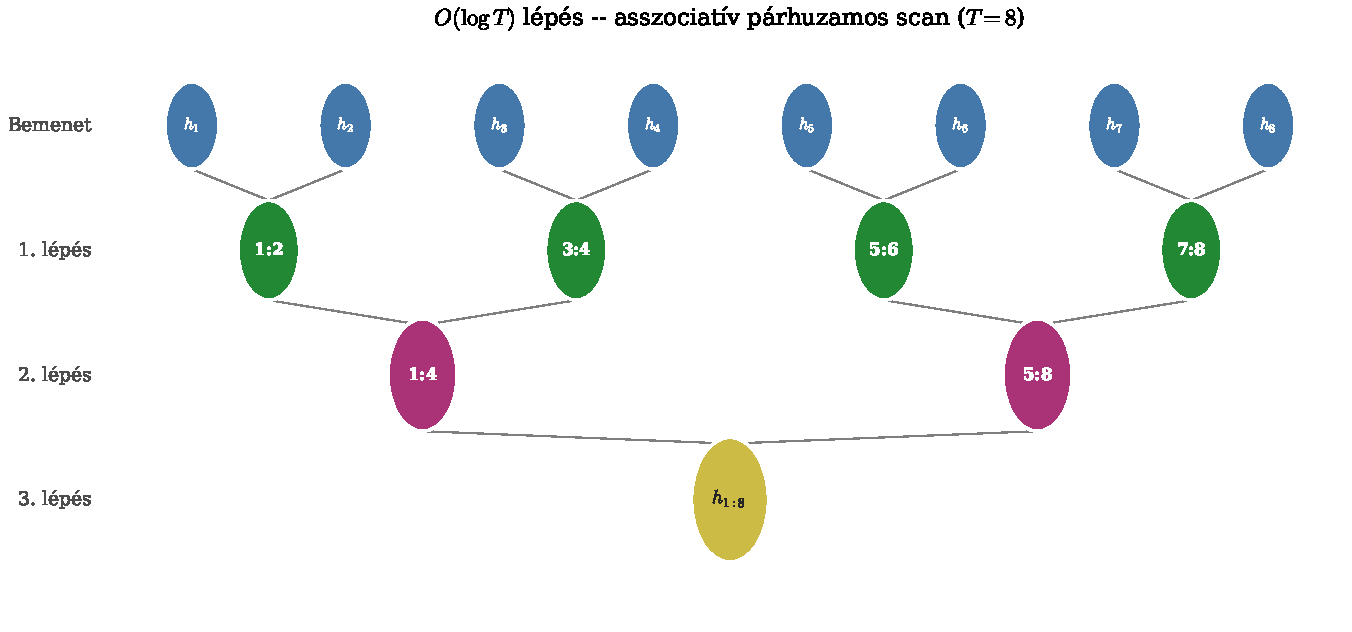
\includegraphics[width=\textwidth]{images/fig09_parallel_scan_hu.pdf}
  \caption{A Blelloch-féle párhuzamos prefix-scan vizualizációja 8 elemű
           szekvencián. Minden lépésben a $step$-nyi távolságú két elem
           kombinálódik.
           $\log_2 T = 3$ lépés után minden $h_t$ tartalmazza az előzmény-összesítést.
           Ez teszi lehetővé a szekvenciális állapotfrissítés hatékony GPU-s
           párhuzamosítását.}
  \label{fig:parallel_scan}
\end{figure}

\subsection{Összegzés és reziduál kapcsolat}

A Kalman-állapot-sorozat és a kapuzás kombinálja a kimenetet:
\begin{equation}
    y_\text{KC} = W_\text{out}(\mu \odot \text{gate}),
\end{equation}
ahol $\mu = (h_1, \ldots, h_T) \in \mathbb{R}^{T \times d_\text{inner}}$
az összes időlépés Kalman-állapota, $W_\text{out} \in \mathbb{R}^{d \times d_\text{inner}}$
a kimeneti projekció, és $\odot$ az elem-szintű szorzás.
Egy skalárkapuzással vezérelt reziduál kapcsolat biztosítja a gradiens
átmenő útját:
\begin{equation}
    \text{out} = y_\text{KC} + \sigma(b_\text{res}) \cdot
                 (W_\text{res}\,x - y_\text{KC}),
\end{equation}
ahol $b_\text{res} \in \mathbb{R}$ tanítható skalár, amelyet $-1{,}0$-ra
inicializálunk, így $\sigma(b_\text{res}) \approx 0{,}27$,
$W_\text{res}$ a reziduál projekció, és a kis $\sigma(b_\text{res})$
alaphelyzetben az SSM-ágat részesíti előnyben.

\section{KCMamba verem}
\label{sec:kc_stack}

A verem $N$ rétegből áll, pre-norm elrendezésű LayerNorm rétegekkel,
amelyek megakadályozzák az aktivációs skála sodródását.

A verem végére egy \emph{multi-scale cross-attention} réteget illesztünk.
Ennek oka, hogy a Mamba rekurrens dinamikája a rejtett állapotba a közelmúlt
lépéseit súlyozottan erősebben kódolja, mint a régmúlt szegmenseket.
Hosszú horizontú előrejelzésnél azonban a lassú trendekhez is hozzáférést
kell biztosítani.
A cross-attention lekérdezésként a jelenlegi állapotot összeveti a szekvencia
minden $s$-edik pozíciójából vett mintázatok (key/value) halmazával,
így rövid és hosszú időskálákat egyaránt számításba vesz:
\begin{equation}
    \text{out}[T] = h[T] + \mathrm{MHA}\bigl(h[T],\; h[{::s}],\; h[{::s}]\bigr),
\end{equation}
ahol $h[T] \in \mathbb{R}^{1 \times d}$ a legutolsó időlépés reprezentációja
és egyben a lekérdezés, $h[{::s}] \in \mathbb{R}^{\lfloor T/s \rfloor \times d}$
minden $s$-edik pozícióból vett alminta, amely a lassabb, durvább
időskálát képviseli kulcsként és értékként,
és $\mathrm{MHA}(\text{lekérdezés},\text{kulcs},\text{érték})$ a multi-head
cross-attention a megszokott értelemben~\cite{vaswani2017attention}.
\begin{figure}[H]
  \centering
  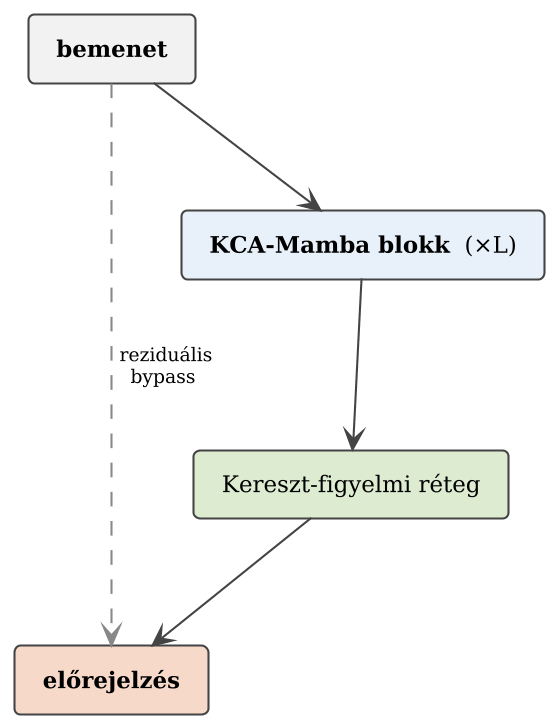
\includegraphics[width=0.55\textwidth, height=0.65\textheight, keepaspectratio]{images/kc_stack_diagram_hu.png}
  \caption{A KCMamba verem (stack) felépítése. A bemenettől a kimenetig az
           input projekció, 2 KC-blokk LayerNorm rétegekkel, output
           normalizáció, majd cross-attention réteg követi egymást a lassú ($s=4$)
           időskála integrálásához.}
  \label{fig:stack_diagram}
\end{figure}
\begin{figure}[H]
  \centering
  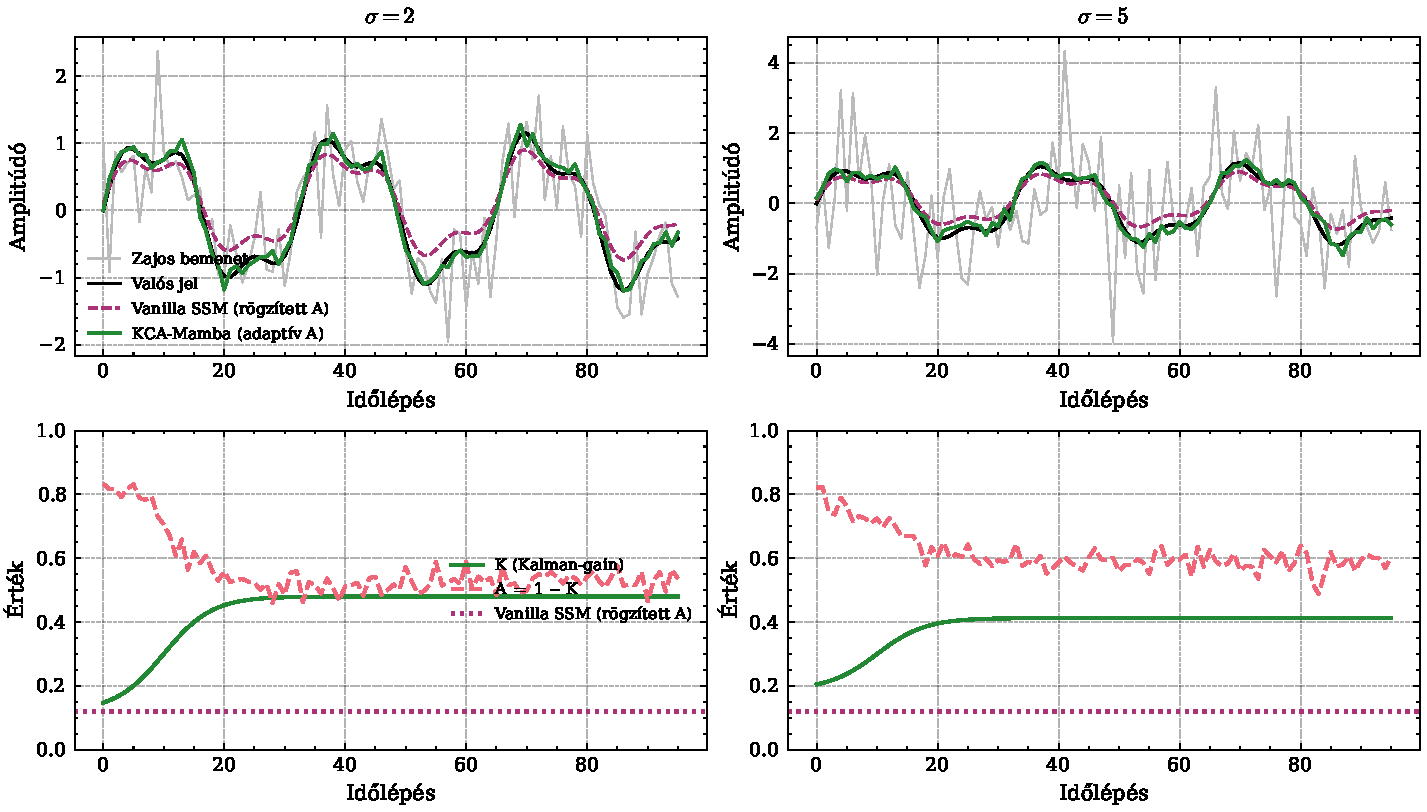
\includegraphics[width=\textwidth]{images/fig11_synth_mamba_hu.pdf}
  \caption{Szintetikus jel szűrése: \textbf{vanilla SSM} (standard Mamba, rögzített $A$)
           vs.\ \textbf{KCMamba} (adaptív $K$-gain) közepes ($\sigma=2$) és erős
           ($\sigma=5$) zajnál.
           \textit{Felső sorok:} az előrejelzett jel a valódihoz képest.
           A KCMamba szorosabban követ zajban is.
           \textit{Alsó sorok:} a tanult $K$-értékek időbeli változása.
           A vanilla SSM $A$-ja rögzített, a KCMamba $A$-ja adaptívan nő zajjal.}
  \label{fig:synth_mamba}
\end{figure}

\begin{figure}[H]
  \centering
  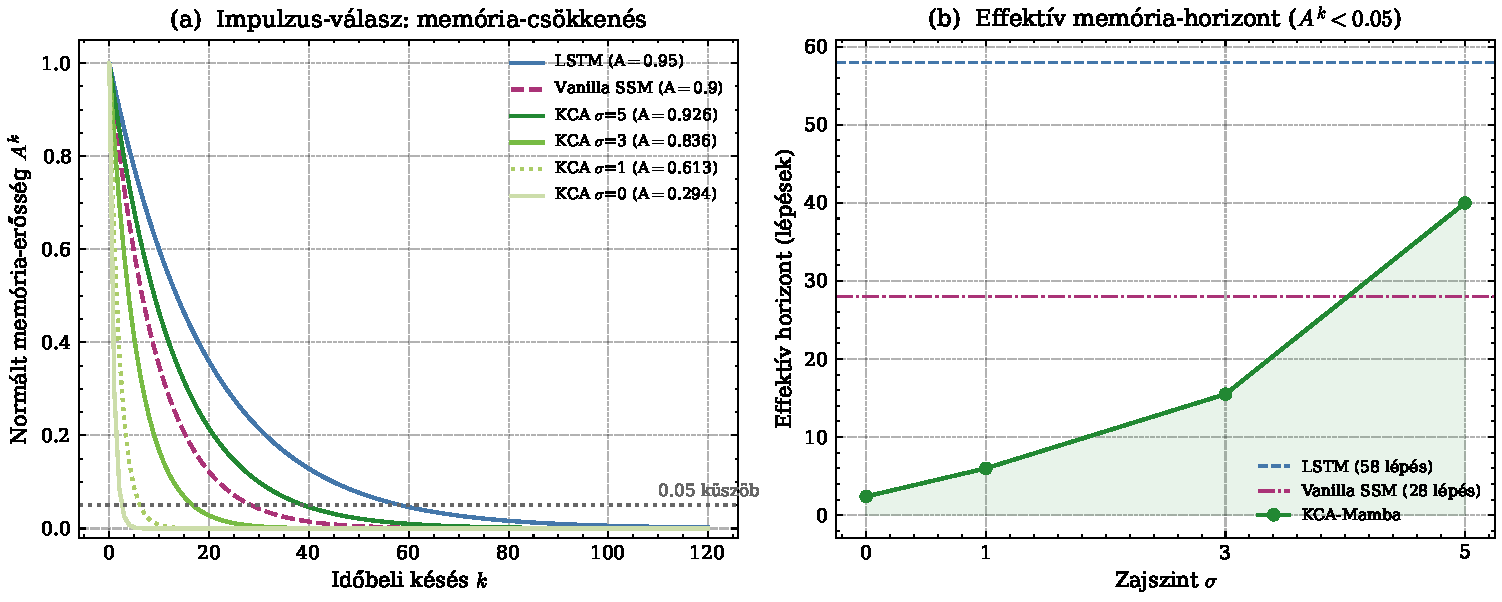
\includegraphics[width=\textwidth]{images/fig13_memory_retention_hu.pdf}
  \caption{\textbf{Bal:} Impulzus-válasz függvény: az állapot exponenciális csökkenése
           $h_k = A^k$ a $k$ késleltetés függvényében. A KCMamba $A$-értéke adaptívan
           nő a zajszinttel ($0.294 \to 0.926$), ezzel a memória-horizont
           is növekszik.
           \textbf{Jobb:} Effektív memória-horizont (az a lépésszám, ameddig
           $A^k > 5\%$) a zajszint függvényében. Az LSTM és vanilla SSM
           rögzített horizonttal rendelkeznek, a KCMamba zajban automatikusan
           hosszabb memóriát tart fenn.}
  \label{fig:memory_retention}
\end{figure}

\section{Paraméterkomplexitás}

\begin{table}[H]
    \centering
    \begin{tabular}{|l|r|r|r|}
        \hline
        \textbf{Modell} & \textbf{Paraméterek (k)} & \textbf{Rétegek} & \textbf{Állapotméret} \\
        \hline\hline
        LSTM            & 71{,}7 & 1 & 128 \\
        Fair Mamba      & 53{,}2 & 2 & H=4, D=32 \\
        KCMamba       & 46{,}1 & 2 & H=4, D=32 \\
        \hline
    \end{tabular}
    \caption{A kísérletekben használt modellek paraméterkomplexitása
             (medium méretkonfiguráció). A KCMamba kevesebb paraméterrel
             rendelkezik, mint a Fair Mamba, mivel a $Q_\text{net}/R_\text{net}/K_\text{net}$
             alhálózatok az SSM-blokkokból az erőforrásokat átirányítják.}
    \label{tab:params}
\end{table}

\newpage
\section{Összehasonlítás a standard Mamba-val}

A legfontosabb architekturális különbség a standard (vanilla) SSM és
a KCMamba között az $A$ felejtési faktor kezelésében keresendő.
A standard Mamba~\cite{gu2023mamba} az $A$ mátrixot a $\Delta$ időléptékű
paraméteren keresztül tanulja, de ez a reprezentáció nem különíti el a
jel- és zajkomponenst: $\Delta$ egyszerre jelöli ki az adatstruktúra
tanulási dinamikáját \emph{és} a zajszűrést.

A KCMamba ezt a kettősséget bontja meg egy explicit $Q/R$
zajtartomány-modell bevezetésével.
A $K = Q/(Q+R)$ arány határozza meg, hogy az állapotfrissítés az
aktuális mérésre vagy az előzmény-állapotra támaszkodik-e erősebben.
Magas zaj mellett ($\sigma=5$) $K \to 0.073$, azaz $A = 0.927$: a modell
erős memóriát tart fenn, és kiszűri a zajos méréseket
(erős szűrési mód).
Alacsony zaj mellett ($\sigma=0$) $K = 0.706$, és a modell az aktuális
megfigyelést követi (\emph{innovációs mód}).

Ezt a szintetikus teszten a \ref{fig:synth_mamba}.\ ábra demonstrálja.
A standard SSM rögzített $A=0.88$ értékkel dolgozik mindkét zajszinten,
míg a KCMamba $A$-ja a zajszinttel arányosan módosul (\ref{fig:memory_retention}.\ ábra).

\newpage
\section{Rendszerarchitektúra}
\label{sec:system_arch}

A KCMamba egy hexagonálisan strukturált kereskedési rendszerbe épül be.
A \ref{fig:system_arch}.\ ábra a főbb komponenseket mutatja:

\begin{figure}[H]
  \centering
  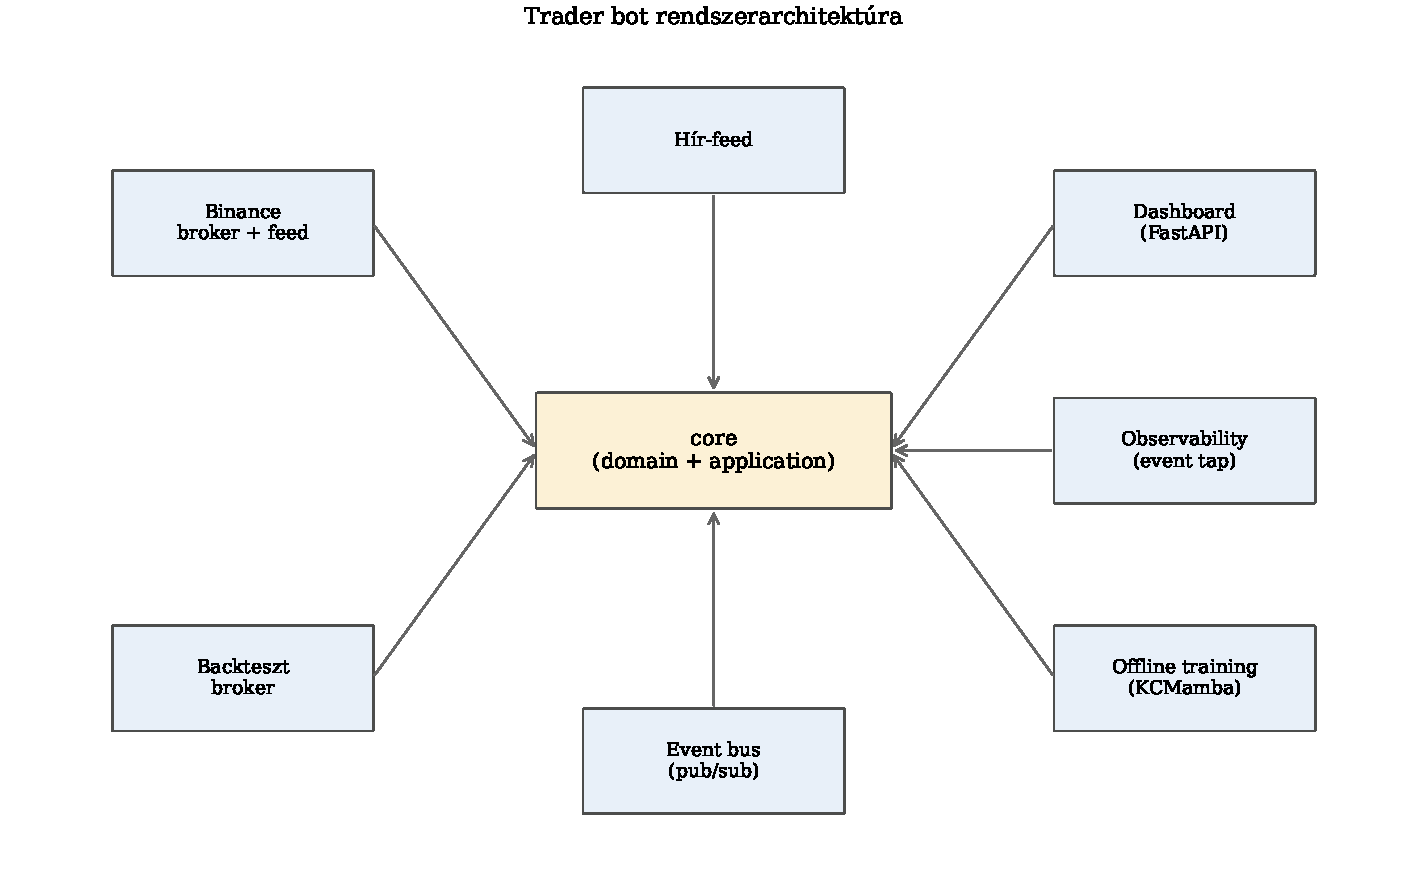
\includegraphics[width=\textwidth]{images/fig14_system_arch_hu.pdf}
  \caption{A KCMamba alapú kereskedési rendszer hexagonális architektúrájának
           áttekintése. A \textbf{Core} csomag tartalmazza a TradingEngine-t
           (pipeline: állapotbecslés $\to$ predikció $\to$ szignál $\to$ kockázat
           $\to$ végrehajtás), a domain modelleket és az alkalmazásportokat.
           A külső adapterek (Infrastructure, Web, Testing, Offline Training,
           Observability, Analytics) kizárólag az interfészeken ($\texttt{IEventBusPort}$,
           $\texttt{IBrokerGatewayPort}$ stb.) keresztül kommunikálnak a Core-ral.}
  \label{fig:system_arch}
\end{figure}

% ─────────────────────────────────────────────────────────────────────────────
\section{Modul- és osztályszerkezet}
\label{sec:module_structure}
% ─────────────────────────────────────────────────────────────────────────────

A forráskód négy fő csomagra oszlik. A \texttt{core/} nem hivatkozik
egyetlen adapterre sem. Az \texttt{adapters/} kód kizárólag a
\texttt{ports.py} interfészeken keresztül éri el.

\begin{table}[H]
  \centering
  \footnotesize
  \renewcommand{\arraystretch}{1.25}
  \begin{tabular}{|l|p{4.2cm}|p{6.3cm}|}
    \hline
    \textbf{Csomag} & \textbf{Modul / osztály} & \textbf{Felelősség} \\
    \hline\hline
    \multirow{4}{*}{\texttt{core/domain/}}
      & \texttt{models.py}      & Adattípusok: \texttt{Candle}, \texttt{Position}, \texttt{Order}, \texttt{Fill} \\
      & \texttt{strategy.py}    & \texttt{ThresholdStrategy}: Buy/Sell jelzéslogika,
                                  \texttt{min\_edge}, \texttt{max\_sigma} szűrők \\
      & \texttt{risk.py}        & \texttt{RiskPolicy}: kockázati szabálykészlet
                                  (MaxQty, Stop-loss, napi veszteség-limit) \\
      & \texttt{events.py}      & Domain-események: \texttt{PriceEvent},
                                  \texttt{SignalEvent}, \texttt{FillEvent} \\
    \hline
    \multirow{5}{*}{\texttt{core/application/}}
      & \texttt{engine.py}      & \texttt{TradingEngine}: fő pipeline-orkesztrálő,
                                  belső állapotgép a kereskedési ciklushoz \\
      & \texttt{execution.py}   & Megbízás-összeállítás, méretszámítás és
                                  \texttt{IBrokerGatewayPort}-ra küldés \\
      & \texttt{ports.py}       & Absztrakt interfészek:
                                  \texttt{IEventBusPort}, \texttt{IBrokerGatewayPort},
                                  \texttt{IMarketFeedPort}, \texttt{ITimeSourcePort} \\
      & \texttt{stages.py}      & Pipeline lépések: \texttt{PredictionStage},
                                  \texttt{SignalStage}, \texttt{RiskStage},
                                  \texttt{ExecutionStage} \\
      & \texttt{stores.py}      & In-memory állapot: \texttt{PositionStore},
                                  \texttt{SignalStore}, \texttt{EquityStore} \\
    \hline
    \multirow{4}{*}{\texttt{core/ml/}}
      & \texttt{kc\_mamba.py}         & \texttt{KCMambaModel}: PyTorch modul,
                                          \texttt{forward(x)} → előrejelzés \\
      & \texttt{mamba\_kalman.py}      & \texttt{KCMambaBlock}: Kalman-szűrő réteg,
                                          párhuzamos prefix-scan \\
      & \texttt{services.py}           & \texttt{MLService}: modellbetöltés,
                                          online frissítés, előrejelzés-gyorsítótár \\
      & \texttt{feature\_engineering.py} & OHLCV → jellemzővektor transzformáció,
                                            normalizáció, csúszóablak \\
    \hline
    \multirow{5}{*}{\texttt{adapters/}}
      & \texttt{binance\_broker.py}    & \texttt{BinanceBroker}: élő megbízás-végrehajtás
                                          REST API-n \\
      & \texttt{binance\_feed.py}      & \texttt{BinanceFeed}: WebSocket árfolyam-stream,
                                          reconnect logika \\
      & \texttt{event\_bus.py}         & \texttt{InMemoryEventBus}: aszinkron,
                                          \texttt{asyncio}-alapú eseménytovábbítás \\
      & \texttt{broker.py} (testing)   & \texttt{PaperBroker}, \texttt{SimulationWallet}:
                                          szimulált végrehajtás visszateszteléshez \\
      & \texttt{dashboard.py} (web)    & \texttt{DashboardServer}: aiohttp HTTP/WS
                                          szerver, REST JSON végpontok \\
    \hline
  \end{tabular}
  \caption{A rendszer modul- és osztályszerkezete. Minden osztály kizárólag a
           saját csomagjának adattípusaira és interfészeire támaszkodik.
           A keresztirányú függőségeket a \texttt{ports.py} absztrakciói
           közvetítik.}
  \label{tab:module_structure}
\end{table}
